\documentclass[12pt, a4paper]{article}
\usepackage{array}
\usepackage{caption}
\usepackage{float}
\usepackage[left=2cm, right=2cm, top=2cm, bottom=2cm]{geometry}
\usepackage{graphicx}
\usepackage{multirow}
\usepackage{subcaption}
\usepackage{xeCJK}

\setCJKmainfont[AutoFakeBold=1.5]{新細明體}
\renewcommand{\arraystretch}{1.2}

\title{
  \vspace{-1cm}
  Network Administration/System Administration\\
  (NTU CSIE, Spring 2024)\\
  Lab 10 - Wireless
}
\author{\Large B12902110 呂承諺}

\begin{document}
  \maketitle
  \section{尋找目標AP}
  \subsection{SSID and BSSID}
  The BSSID can be directly obtained in Wi-Fi details.
  \begin{table}[H]
    \begin{tabular}{|cc|}
      \hline
      \textbf{SSID}   & \textbf{BSSID}    \\\hline
      nasa-lab10-2.4G & 30:87:d9:31:97:69 \\
      nasa-lab10-5G   & 30:87:d9:f1:97:6c \\\hline
    \end{tabular}
  \end{table}

  \begin{figure}[H]
    \begin{subfigure}{0.4\textwidth}
      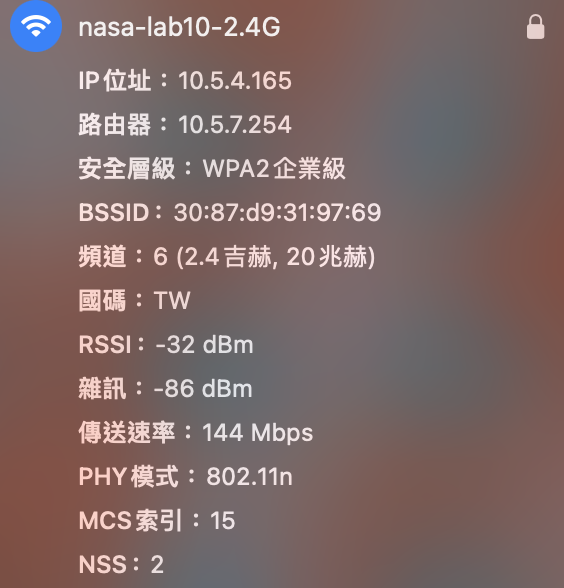
\includegraphics[width=\textwidth]{2.4G_closest.png}
      \caption{2.4~GHz}
    \end{subfigure}
    \begin{subfigure}{0.4\textwidth}
      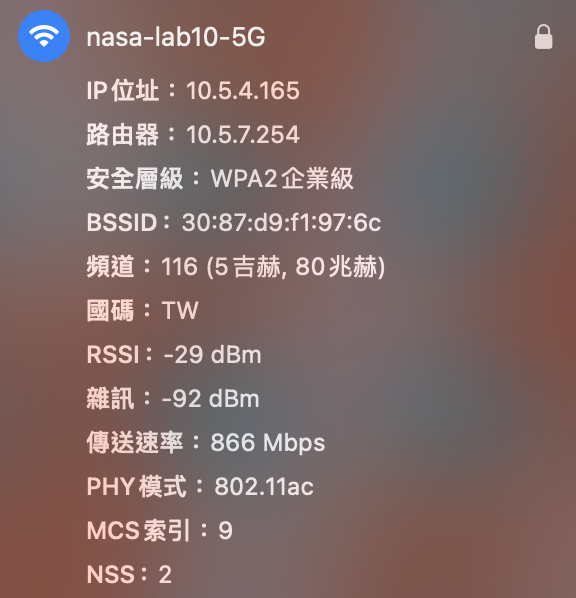
\includegraphics[width=\textwidth]{5G_closest.png}
      \caption{5~GHz}
    \end{subfigure}
  \end{figure}

  \pagebreak
  \subsection{AP location}
  We measure the RSSI of nasa-lab10-5G when standing right beside every AP.
  \begin{table}[H]
    \begin{tabular}{|cc|}
      \hline
      \textbf{AP location} & \textbf{RSSI} \\\hline
       R204 & -29~dBm \\
       R208 & -63~dBm \\
       R214 & -81~dBm \\\hline
    \end{tabular}
  \end{table}
  \begin{figure}[H]
    \begin{subfigure}{0.32\textwidth}
      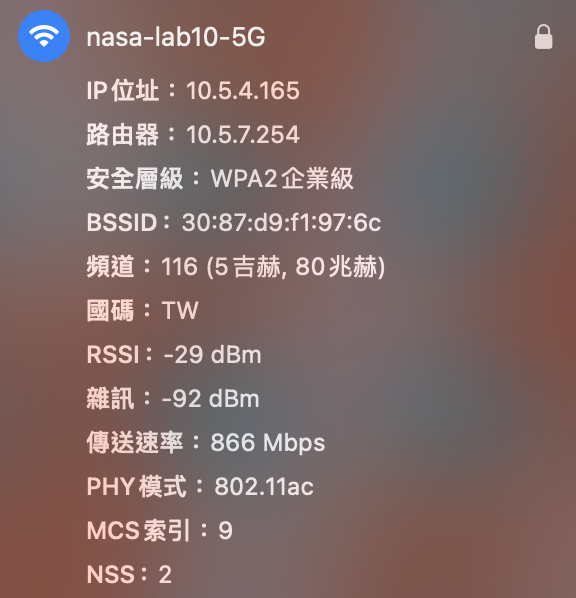
\includegraphics[height=5.6cm]{5G_closest.png}
      \caption{R204}
    \end{subfigure}
    \hfill
    \begin{subfigure}{0.32\textwidth}
      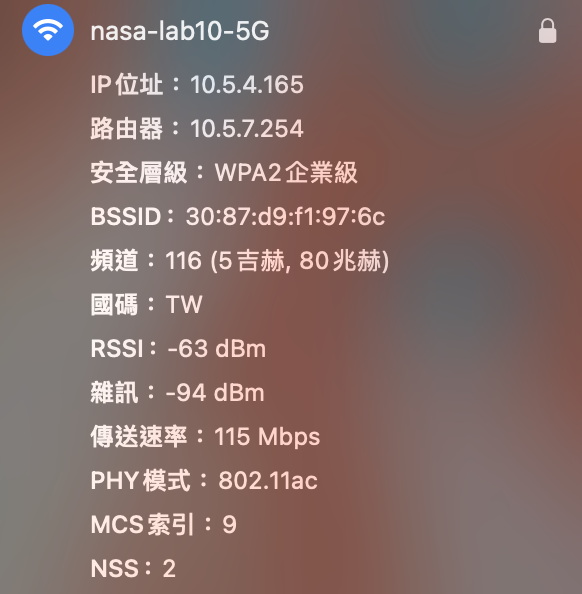
\includegraphics[height=5.6cm]{5G_R208.png}
      \caption{R208}
    \end{subfigure}
    \hfill
    \begin{subfigure}{0.32\textwidth}
      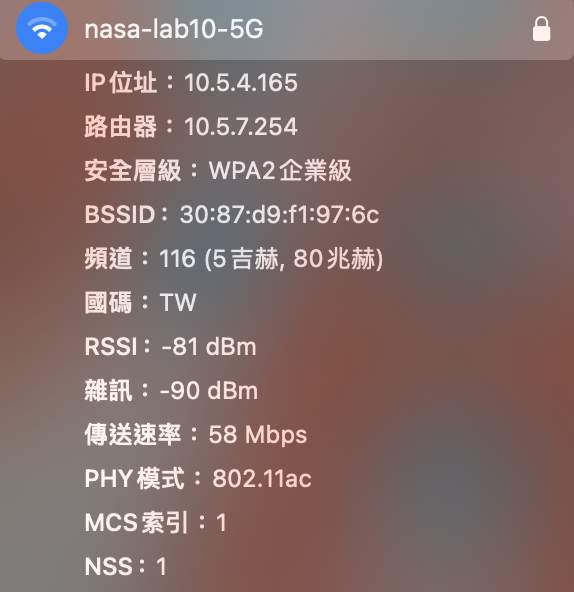
\includegraphics[height=5.6cm]{5G_R214.png}
      \caption{R214}
    \end{subfigure}
  \end{figure}

  The signal is the strongest while standing next to the AP in R204, so we infer that
  the AP is the one in R204.

  \section{測量數據}
  \textbf{Terms}
  \begin{itemize}
    \item \textbf{RSSI}: Received signal strength indicator. The amount of
    power of a received signal. It's measured in dBm (decibel-milliwatts),
    decibels relative to one milliwatt.
    \item \textbf{SNR}: Signal-to-noise ratio. A lower value means clearer signal and less noise. It's measured in dB (decibels).
    \item \textbf{Transmission rate}: Maximum theoretical transmission rate
    calculated from the current negotiated transfer scheme. Signal strength and
    SNR could affect which scheme is chosen. It's usually measured in Mbps
    (Megabits per second).
  \end{itemize}

  \noindent\textbf{Result}
  \begin{table}[H]
    \begin{tabular}{|ccccc|}
      \hline
      \textbf{Frequency} & \textbf{Condition} & \textbf{RSSI} &
      \textbf{SNR} & \textbf{Transmission rate} \\\hline
      \multirow{3}{*}{2.4~GHz} &
        Next to AP             & -32~dBm & 54~dB & 144~Mbps \\
      & Farthest line of sight & -47~dBm & 43~dB & 144~Mbps \\
      & Behind wall            & -44~dBm & 46~dB & 144~Mbps \\\hline
      \multirow{3}{*}{5~GHz} &
        Next to AP             & -29~dBm & 63~dB & 866~Mbps \\
      & Farthest line of sight & -54~dBm & 36~dB & 130~Mbps \\
      & Behind wall            & -55~dBm & 39~dB & 585~Mbps \\\hline
    \end{tabular}
  \end{table}
  \begin{figure}[H]
    \begin{subfigure}{0.32\textwidth}
      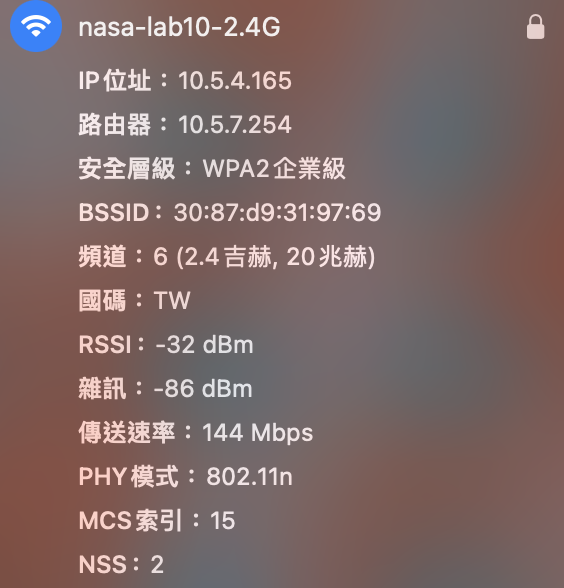
\includegraphics[height=5.6cm]{2.4G_closest.png}
      \caption{2.4~GHz, next to AP}
    \end{subfigure}
    \hfill
    \begin{subfigure}{0.32\textwidth}
      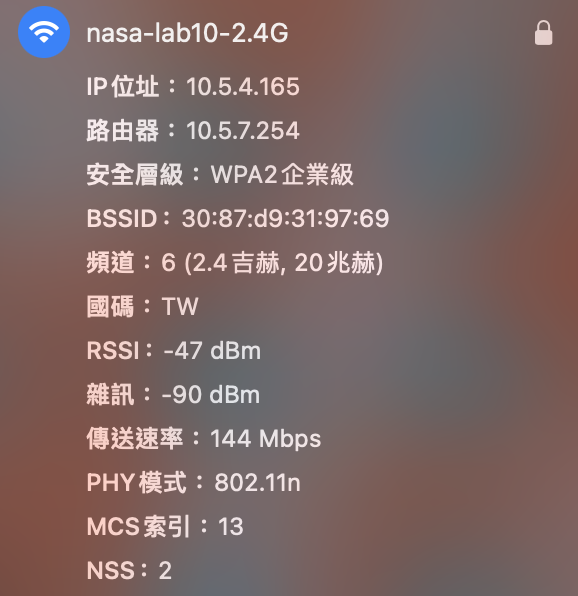
\includegraphics[height=5.6cm]{2.4G_farthest.png}
      \caption{2.4~GHz, farthest line of sight}
    \end{subfigure}
    \hfill
    \begin{subfigure}{0.32\textwidth}
      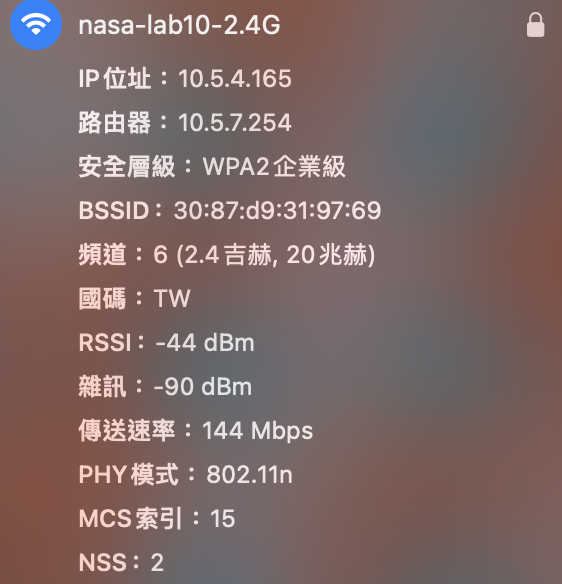
\includegraphics[height=5.6cm]{2.4G_wall.png}
      \caption{2.4~GHz, behind wall}
    \end{subfigure}
    \begin{subfigure}{0.32\textwidth}
      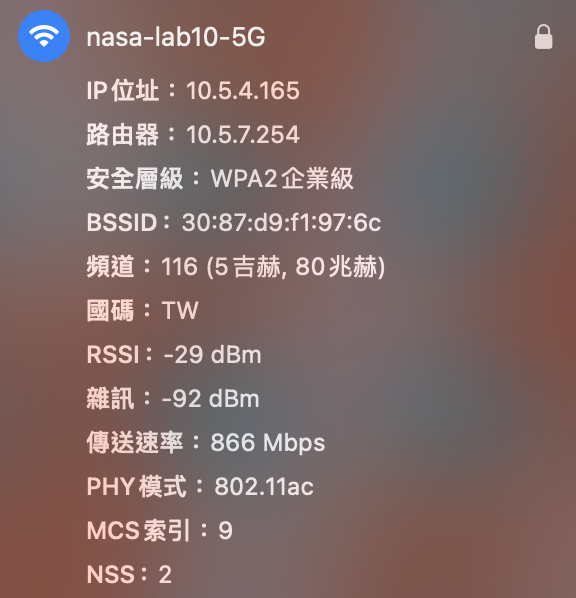
\includegraphics[height=5.6cm]{5G_closest.png}
      \caption{5~GHz, next to AP}
    \end{subfigure}
    \hfill
    \begin{subfigure}{0.32\textwidth}
      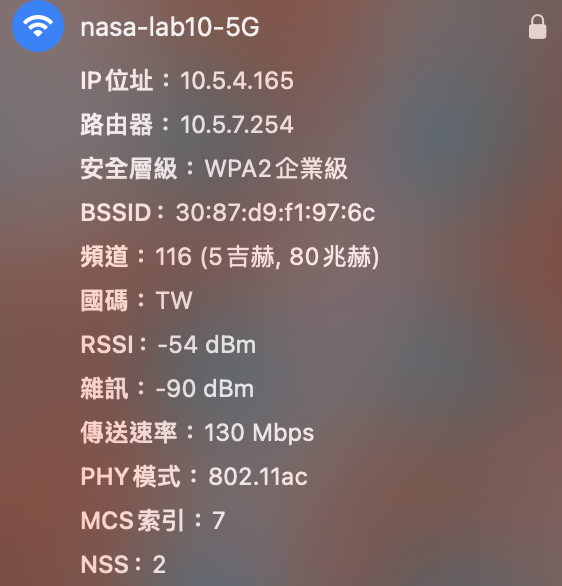
\includegraphics[height=5.6cm]{5G_farthest.png}
      \caption{5~GHz, farthest line of sight}
    \end{subfigure}
    \hfill
    \begin{subfigure}{0.32\textwidth}
      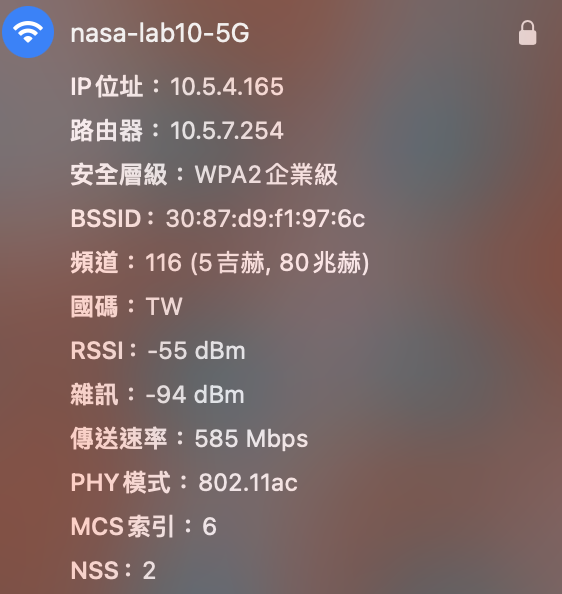
\includegraphics[height=5.6cm]{5G_wall.png}
      \caption{5~GHz, behind wall}
    \end{subfigure}
  \end{figure}

  \section{分析數據}
  Distance mainly affects the RSSI, which in turn determines the transmission rate.
  The farther away the receiver is to the AP, the less power it would receive, and
  the transmission rate would drop as well. Noise is not influenced by distance
  according to our experiment.

  5~GHz signals can only achieve the maximum transmission rates if the signal is
  fairly strong; even if the signal strength drops by a little, the maximum
  transmission rate will drop. On the other hand, 2.4~GHz signals can still operate
  at its maximum rate if the signal drops by around 10 dB. However note that
  2.4~GHz transmission rates are slower than that of 5~GHz.

  When a wall is between the transmitter and the receiver, 5~GHz signals degrades
  more than 2.4~GHz signals. This is because waves with longer wavelengths can penetrate through obstacles better.
\end{document}
